\section{Моделирование предметной области и разработка функциональных
требований}

\subsection{Сенсоры}

Для получения информации об окружающей среде используются различные сенсоры.

\subsubsection{Lidar}
Сенсор Lidar выдаёт 2D снимок помещения -- облако точек в двумерной плоскости.
Используя облако точек, и зная позицию в которой снимок облака был совершён,
возможно реконструировать карту окружающего пространства на сетке. Если провести
отметить все клетки через которые прошёл луч за пустые, и отметить последнюю
клетку которую луч зацепил в качестве отмеченной, то получается 

\begin{figure}[h]
\centering
	\fbox{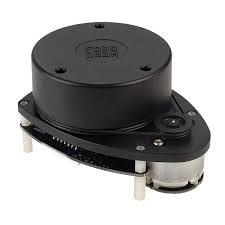
\includegraphics[width=9cm]{2d_lidar}}
\caption{2D Lidar}
\end{figure}

\subsubsection{IMU}
Сенсор IMU выдаёт угловое и линейное ускорение

\subsubsection{GPS}
Сенсор GPS выдаёт глобальную позицию в мировых координатах. Для того чтобы
привести координаты на плоскость используем UTM развёртку для локальной
местности.

\subsection{Общие сведения и требования к работе программного средства}
- Построение карты
- Следование маршруту
- Конфигурация 

\subsection{Описание функциональности программного средства}

\todo{USECASE диаграмма}

\subsection{Спецификация функциональных требований}

- Моделируем навигацию

- Occupancy grid

- Надо переместится в указанную точку на карте
- Способ указывания точки на карте


\todo{ Если цель переместится в указанную точку, для этого надо построить
маршрут, чтобы построить маршрут нужна карта, чтобы построить карту используем
позицию и показания с сенсоров и метод SLAM }

\subsection{Функциональные требования}
    - Функциональные требования
        - Получение данных с датчиков
        - **требования** Спецификация функциональных требования/Разработка
          спецификации фун. треб. + разработка тех. требований
